% Number 478
% UFPM Normal
% Accel. elevator: v down, slowing down - find T
% MIT

% Watermark
\AddToShipoutPicture*{\BackgroundPic}

\addtocounter {ProbNum} {1}

\begin{floatingfigure}[r]{.2\textwidth}
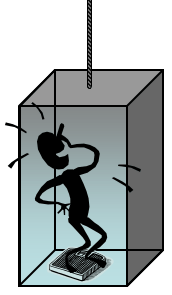
\includegraphics[scale=.6]{/Users/jgates/desktop/latex/pics/scaleinelevator1}
\end{floatingfigure}
 
{\bf \Large{\arabic{ProbNum}}} A 1700 kg elevator contains a 76 kg physicist standing on a scale. The elevator is moving downwards at a rate of ${4.1~\tfrac{m}{s}}$ and slowing down at a rate of ${2.5~\tfrac{m}{s^2}}$.

\bigskip
What is the tension in the cable?


%\begin{center}
%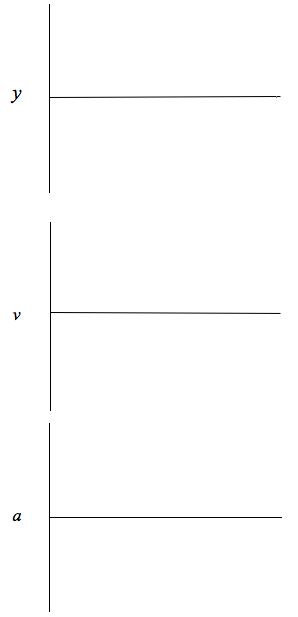
\includegraphics[scale=.85]{/Users/jgates/desktop/latex/pics/blankyvagraphstack.png}
%\end{center}


\vfill
\newpage
